
\begin{figure}
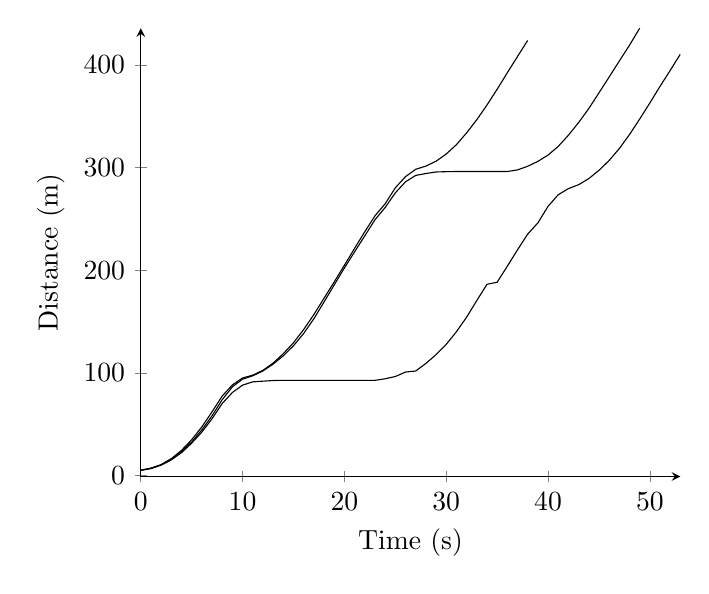
\begin{tikzpicture}
\begin{axis}[
legend style={anchor=west},
axis x line=bottom,
axis y line=left,
ymin=-1,
xlabel=Time (s),
ylabel=Distance (m),
]
\addplot[] coordinates {
(0, 5.1)
(1, 6.69303435794)
(2, 10.0552175429)
(3, 15.1565769477)
(4, 22.2384550413)
(5, 31.4882965597)
(6, 42.2893118176)
(7, 55.3226277287)
(8, 70.1283037292)
(9, 80.8867706297)
(10, 88.0756863912)
(11, 91.2211859886)
(12, 91.90163235)
(13, 92.5358591542)
(14, 92.7123251886)
(15, 92.7123251886)
(16, 92.7123251886)
(17, 92.7123251886)
(18, 92.7123251886)
(19, 92.7123251886)
(20, 92.7123251886)
(21, 92.7123251886)
(22, 92.7123251886)
(23, 92.7123251886)
(24, 94.2294904455)
(25, 96.4442856215)
(26, 100.778688769)
(27, 101.814351466)
(28, 109.138314476)
(29, 117.722293296)
(30, 127.748846634)
(31, 140.060106472)
(32, 154.203889951)
(33, 170.378622624)
(34, 186.277994066)
(35, 188.276298129)
(36, 203.879524269)
(37, 219.794675433)
(38, 235.160214173)
(39, 246.064053183)
(40, 262.213540888)
(41, 273.513880333)
(42, 279.472814001)
(43, 283.297360916)
(44, 289.21772063)
(45, 297.291853257)
(46, 306.911440106)
(47, 318.475357958)
(48, 332.149444655)
(49, 347.24034591)
(50, 362.937290954)
(51, 379.144361228)
(52, 394.665868647)
(53, 410.569931062)
};
\addplot[] coordinates {
(0, 5.1)
(1, 7.08205558845)
(2, 10.5445840002)
(3, 16.3794734145)
(4, 24.4809364524)
(5, 34.8723273118)
(6, 47.3577491635)
(7, 62.0826429908)
(8, 77.4028045407)
(9, 88.2928776022)
(10, 95.0325133104)
(11, 97.7102715983)
(12, 102.484544425)
(13, 109.512239172)
(14, 118.742838738)
(15, 129.344661082)
(16, 142.218723297)
(17, 156.765024348)
(18, 172.70912197)
(19, 188.602555026)
(20, 204.812824753)
(21, 221.317916541)
(22, 237.455140303)
(23, 252.979844152)
(24, 264.670122978)
(25, 280.257341035)
(26, 291.106054659)
(27, 298.303671478)
(28, 301.43227868)
(29, 306.146544919)
(30, 313.200067599)
(31, 322.283617672)
(32, 333.756161656)
(33, 346.559652501)
(34, 360.871285153)
(35, 376.251351805)
(36, 392.34262205)
(37, 408.181358697)
(38, 423.798926573)
};
\addplot[] coordinates {
(0, 5.1)
(1, 7.1506696598)
(2, 10.524638952)
(3, 16.2240841987)
(4, 23.3360430318)
(5, 32.697633148)
(6, 44.4491036579)
(7, 58.1600494656)
(8, 73.8461444279)
(9, 86.4101363573)
(10, 93.8437257624)
(11, 97.12893211)
(12, 101.8606097)
(13, 108.539832858)
(14, 116.652814372)
(15, 126.393898077)
(16, 138.370528499)
(17, 152.72145718)
(18, 169.057055409)
(19, 185.642096296)
(20, 202.150092105)
(21, 217.905350454)
(22, 233.418151974)
(23, 249.132139908)
(24, 261.056869098)
(25, 275.374333291)
(26, 286.090594978)
(27, 292.320706796)
(28, 294.207469484)
(29, 295.684866407)
(30, 295.988687949)
(31, 296.137727391)
(32, 296.137727391)
(33, 296.137727391)
(34, 296.137727391)
(35, 296.137727391)
(36, 296.137727391)
(37, 297.725278116)
(38, 301.257313771)
(39, 306.009297207)
(40, 312.147874803)
(41, 320.598667972)
(42, 331.470724363)
(43, 343.82416272)
(44, 357.456302213)
(45, 372.755577611)
(46, 388.180582012)
(47, 403.804174287)
(48, 419.160505382)
(49, 435.734900077)
};

\end{axis}
\end{tikzpicture}
\label{tik:0:14_V, 15_N, 17_S, 17_S.-60, 19_V}
\caption{0 percent diving with GSC on route $14_V, 15_N, 17_S, 17_S.-60, 19_V$}
\end{figure}
